\documentclass[11pt]{article}
\usepackage[letterpaper,margin=0.85in]{geometry}
\usepackage{graphicx}
\usepackage{booktabs}
\usepackage{array}
\usepackage{float}
\usepackage{caption}
\usepackage{subcaption}
\usepackage{amsmath}
\usepackage{siunitx}
\usepackage[hidelinks]{hyperref}
\usepackage{xcolor}
\usepackage{microtype}
\usepackage{enumitem}
\usepackage{setspace}
\usepackage{fancyhdr}
\usepackage{url}

\IfFileExists{../results/results.tex}{\newcommand{\NObs}{2110}
\newcommand{\NMissing}{0}
\newcommand{\PCOneVar}{92.5\%}
\newcommand{\PCTwoVar}{6.3\%}
\newcommand{\PCTwoCum}{98.8\%}
\newcommand{\NPCOptimal}{1}
\newcommand{\PCOneTop}{QBER}
\newcommand{\PCTwoTop}{VOA\_dB}
\newcommand{\KOptimal}{3}
\newcommand{\LDAAccuracy}{39.2\%}
\newcommand{\TrainN}{1475}
\newcommand{\TestN}{635}
\newcommand{\LDOneTop}{LogSKR}
\newcommand{\LDTwoTop}{QBER}
\newcommand{\LDAMajorityAccuracy}{26.8\%}
\newcommand{\LDAMacroRecall}{32.2\%}
\newcommand{\ClusterARI}{0.650}
\newcommand{\KmeansSilhouette}{0.668}
\newcommand{\WardSilhouette}{0.595}
\newcommand{\RegressionQberRsq}{0.816}
\newcommand{\RegressionLogSkrRsq}{0.748}
\newcommand{\AttenuationCenter}{21.69}
}{
\newcommand{\NObs}{--}\newcommand{\NMissing}{--}
\newcommand{\PCOneVar}{--}\newcommand{\PCTwoVar}{--}\newcommand{\PCTwoCum}{--}
\newcommand{\NPCOptimal}{--}\newcommand{\PCOneTop}{--}\newcommand{\PCTwoTop}{--}
\newcommand{\KOptimal}{--}\newcommand{\LDAAccuracy}{--}\newcommand{\TrainN}{--}\newcommand{\TestN}{--}
\newcommand{\LDOneTop}{--}\newcommand{\LDTwoTop}{--}}

\pagestyle{fancy}
\fancyhf{}
\lhead{M5 Assignment 5.1}
\rhead{Asif Akhtab Ronggon}
\cfoot{\thepage}
\setlength{\headheight}{14pt}
\setstretch{1.03}
\captionsetup{font=small,labelfont=bf}

\title{\textbf{Multivariate Analysis of Quantum Key Distribution Performance\\under Classical-Signal Coexistence}}
\author{Asif Akhtab Ronggon}
\date{September 2026}

\begin{document}
\maketitle

\section{Introduction and Dataset Description}
Quantum key distribution (QKD) systems must maintain low quantum bit error rate (QBER) and a usable secure key rate (SKR) while operating in optical environments that may also carry classical traffic. This report applies multivariate statistical methods to experimental QKD coexistence measurements from the TCD/CONNECT testbed published by Horgan et al. on Zenodo \cite{horgan2026}. The source record contains measurement-level QBER and SKR observations collected under controlled attenuation, classical-signal injection, and fibre-length conditions.

To isolate the effect of injected classical power from the separate effect of added fibre length, this analysis uses the five \SI{0}{km} coexistence conditions: no injected signal (baseline), and injected powers of 3, 7, 9, and \SI{12}{dBm}. The resulting analysis dataset contains \NObs{} measurement-level observations. The quantitative variables are optical attenuation (\texttt{VOA\_dB}), QBER, and secure key rate. Because SKR spans orders of magnitude and reaches zero near link collapse, the transformed variable $\log_{10}(\mathrm{SKR}+1)$ is used in PCA, clustering, and LDA. The categorical grouping variable is the injected-noise condition.

The analysis addresses three complementary questions: (i) what low-dimensional structure explains the joint variation in attenuation, QBER, and SKR; (ii) whether the measurements form natural unsupervised clusters; and (iii) how effectively the quantitative measurements discriminate among the five predefined coexistence conditions.

\section{Data Preprocessing and Exploratory Analysis}
The five CSV files were downloaded directly from the version-2 Zenodo record and combined in R. Required columns, numeric types, finite values, recognized conditions, and nonzero predictor standard deviations were checked before analysis. The dataset contains \NMissing{} missing values across all fields; missing values in required analysis fields cause the script to stop. QBER values outside $[0,1]$ and negative SKR values also cause validation to fail. Zero-SKR observations were retained because they represent physically meaningful key-generation collapse rather than missing data.

For multivariate methods, $\log_{10}(\mathrm{SKR}+1)$ was used to reduce the strong right skew in raw SKR while retaining zeros. The three quantitative variables were standardized to zero mean and unit variance before PCA and clustering so that the analysis was not dominated by their different physical units and numerical scales.

\begin{table}[H]
\centering
\caption{Descriptive statistics by injected classical-signal condition.}
\label{tab:desc}
\small
\IfFileExists{../results/descriptive_table.tex}{\begin{tabular}{lrrrr}
\toprule
Condition & $n$ & Mean QBER & Median SKR (bps) & Zero-SKR (\%) \\
\midrule
Baseline & 471 & 0.0484 &  3,541 & 8.7 \\
3 dBm & 400 & 0.0493 &  5,673 & 13.0 \\
7 dBm & 354 & 0.0467 &  8,400 & 8.2 \\
9 dBm & 319 & 0.0491 &  3,319 & 9.4 \\
12 dBm & 566 & 0.0457 & 91,610 & 22.1 \\
\bottomrule
\end{tabular}
}{Results generated when the R analysis runs.}
\end{table}

Figure~\ref{fig:eda} provides two complementary views of the data. The QBER curves show how error behavior changes with attenuation across coexistence conditions, while the log-SKR curves show the corresponding reduction in usable secure-key throughput. Examining both responses is important: a QKD operating point can exhibit a modest QBER change while the usable key rate is already deteriorating substantially.

\begin{figure}[H]
\centering
\begin{subfigure}[t]{0.49\textwidth}
\centering
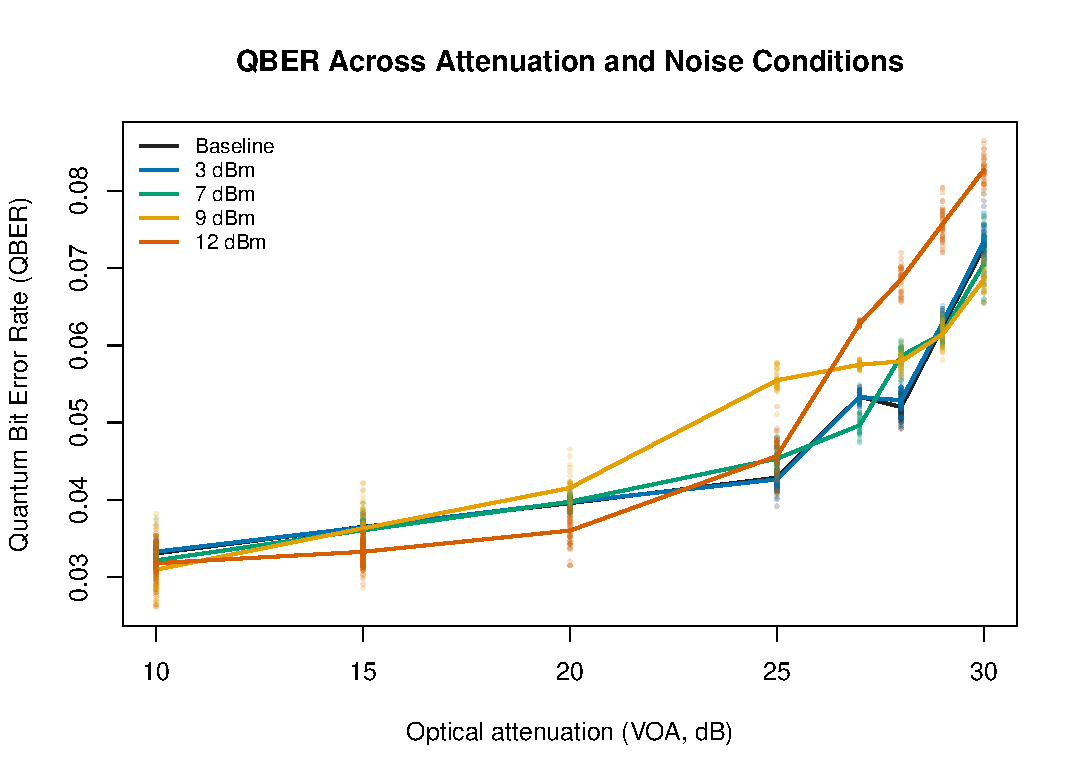
\includegraphics[width=\linewidth]{../figures/03_qber_vs_attenuation.pdf}
\caption{QBER versus attenuation.}
\end{subfigure}\hfill
\begin{subfigure}[t]{0.49\textwidth}
\centering
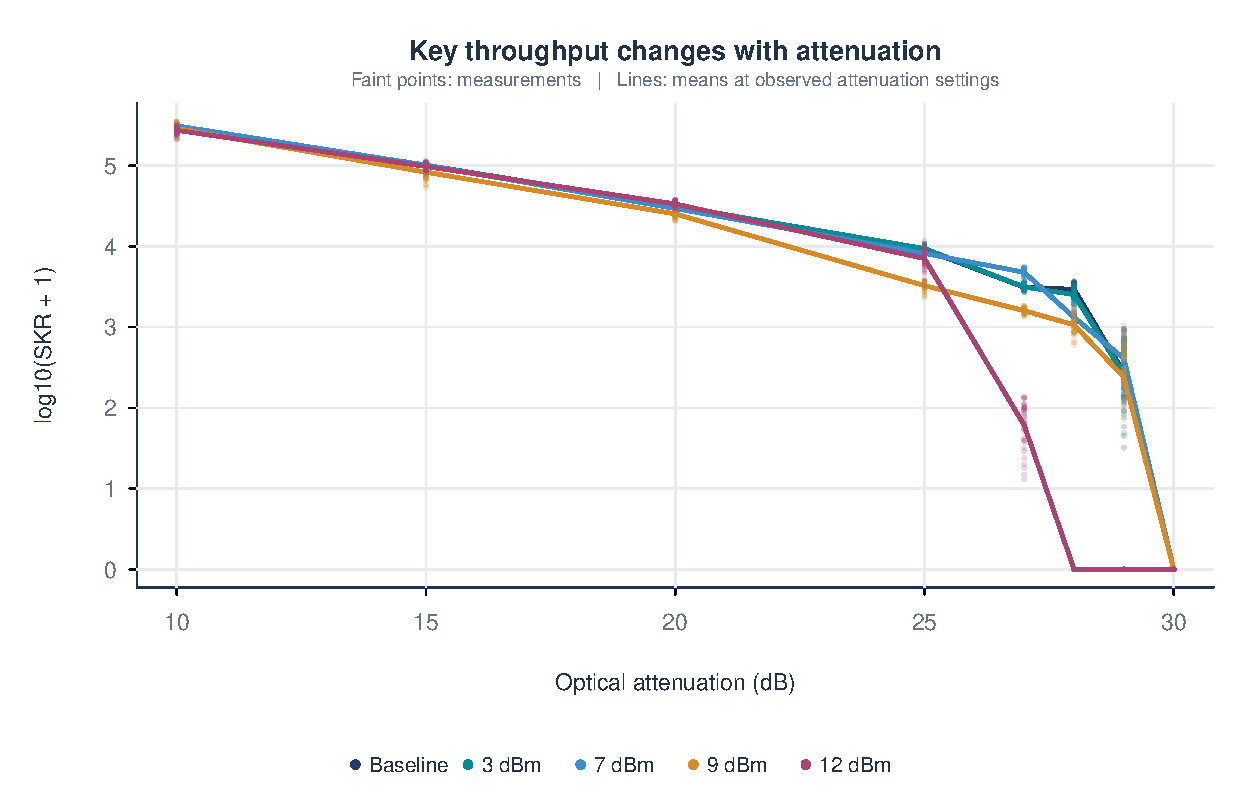
\includegraphics[width=\linewidth]{../figures/04_logskr_vs_attenuation.pdf}
\caption{Log-SKR versus attenuation.}
\end{subfigure}
\caption{Exploratory views of QKD performance across injected-signal conditions. Lines show condition-wise means at each attenuation setting; faint points show individual measurements.}
\label{fig:eda}
\end{figure}

The scatterplot matrix and correlation matrix (Figure~\ref{fig:corr}) are used to assess pairwise relationships before applying multivariate methods. These visualizations motivate PCA because several variables exhibit substantial dependence rather than contributing fully independent information.

\begin{figure}[H]
\centering
\begin{subfigure}[t]{0.49\textwidth}
\centering
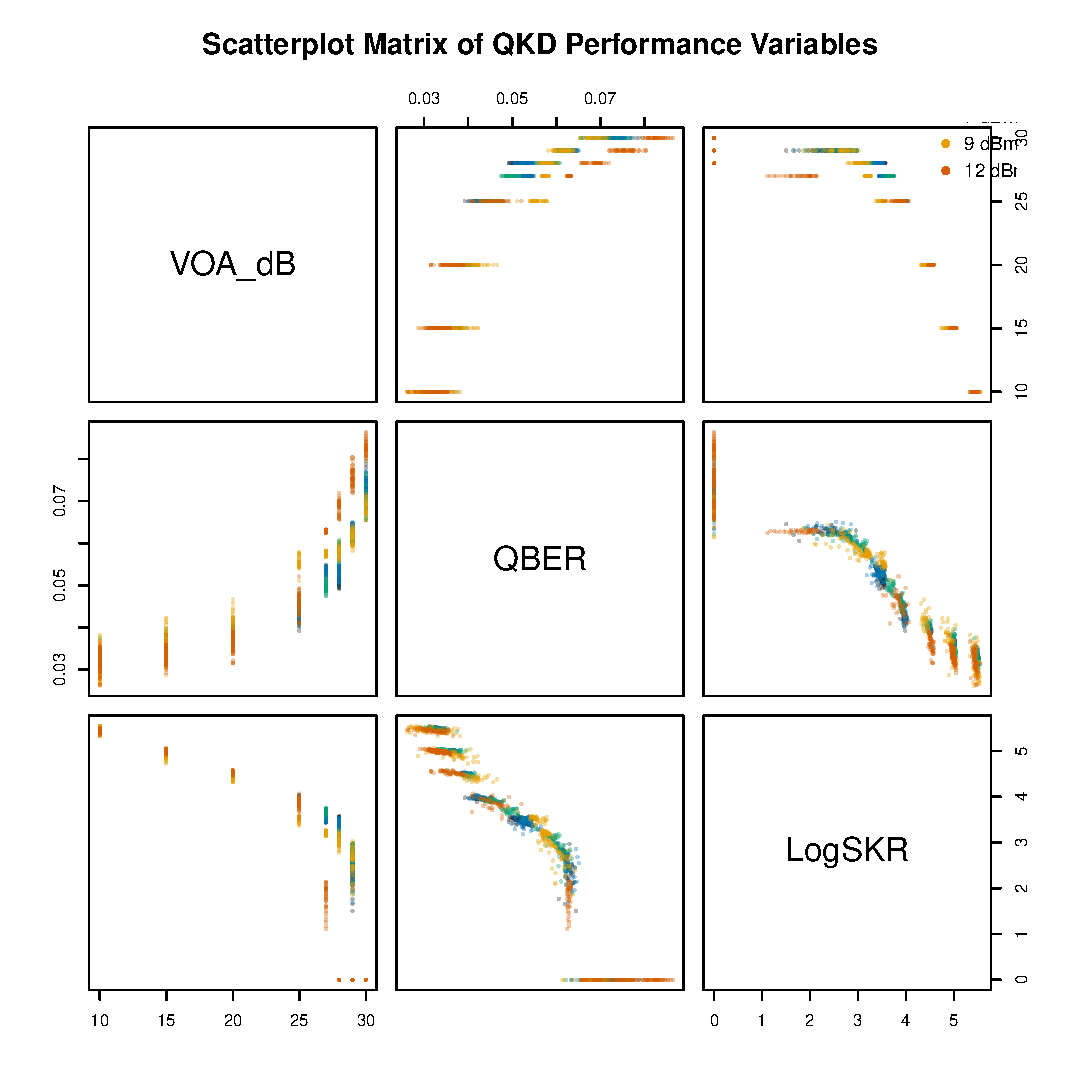
\includegraphics[width=\linewidth]{../figures/01_scatterplot_matrix.pdf}
\caption{Scatterplot matrix.}
\end{subfigure}\hfill
\begin{subfigure}[t]{0.49\textwidth}
\centering
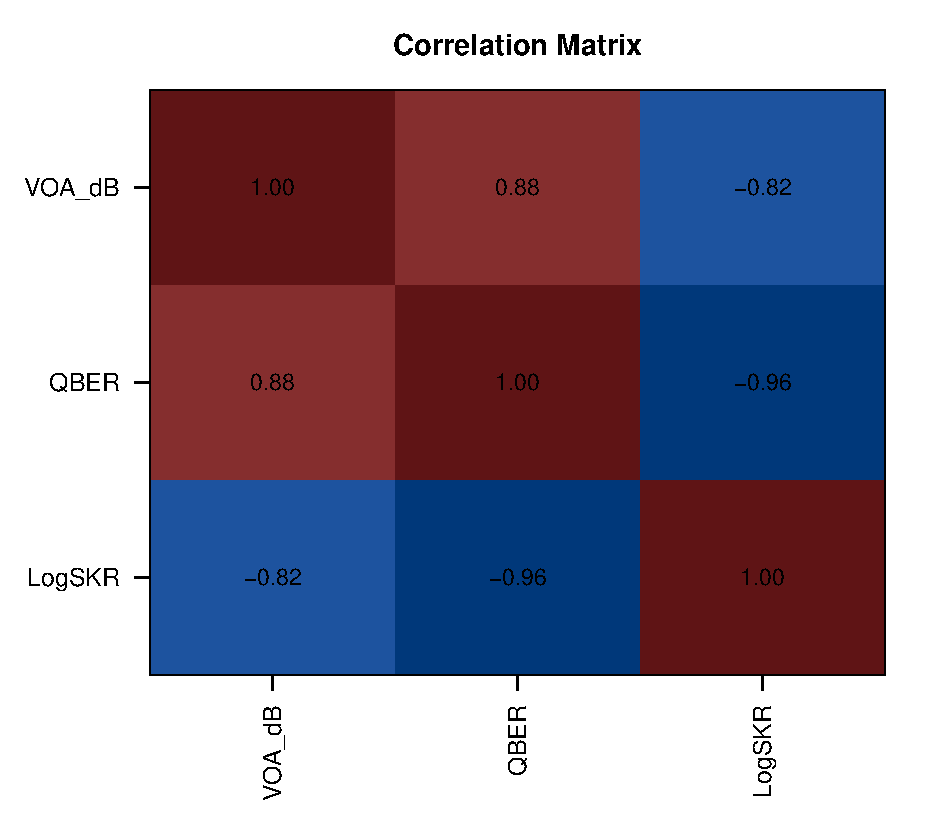
\includegraphics[width=\linewidth]{../figures/02_correlation_matrix.pdf}
\caption{Correlation matrix.}
\end{subfigure}
\caption{Pairwise structure among attenuation, QBER, and transformed secure key rate.}
\label{fig:corr}
\end{figure}

\section{Principal Component Analysis}
PCA was performed on the standardized variables $\{\mathrm{VOA},\mathrm{QBER},\log_{10}(\mathrm{SKR}+1)\}$. If $\mathbf{Z}$ denotes the standardized data matrix, PCA finds orthogonal directions $\mathbf{w}_j$ that maximize projected variance, with scores $\mathbf{t}_j=\mathbf{Z}\mathbf{w}_j$.

\begin{table}[H]
\centering
\caption{PCA eigenvalues and explained variance.}
\label{tab:pca_var}
\small
\IfFileExists{../results/pca_table.tex}{\begin{tabular}{lrrr}
\toprule
Component & Eigenvalue & Variance (\%) & Cumulative (\%) \\
\midrule
PC1 & 2.774 & 92.5 & 92.5 \\
PC2 & 0.190 & 6.3 & 98.8 \\
PC3 & 0.036 & 1.2 & 100.0 \\
\bottomrule
\end{tabular}
}{Results generated when the R analysis runs.}
\end{table}

PC1 explains \PCOneVar{} of standardized variance and PC2 explains an additional \PCTwoVar{}, for \PCTwoCum{} cumulatively. Using an 80\% cumulative-variance criterion requires \NPCOptimal{} principal component(s). The largest absolute loading on PC1 is associated with \texttt{\PCOneTop}, while the strongest loading on PC2 is \texttt{\PCTwoTop}. The loading table in Table~\ref{tab:pca_load} makes the direction and relative magnitude of each contribution explicit.

\begin{table}[H]
\centering
\caption{PCA loadings for the standardized quantitative variables.}
\label{tab:pca_load}
\small
\IfFileExists{../results/pca_loadings_table.tex}{\begin{tabular}{lrrr}
\toprule
Variable & PC1 & PC2 & PC3 \\
\midrule
VOA\_dB & 0.561 & 0.808 & -0.177 \\
QBER & 0.591 & -0.242 & 0.770 \\
LogSKR & -0.580 & 0.537 & 0.613 \\
\bottomrule
\end{tabular}
}{Results generated when the R analysis runs.}
\end{table}

\begin{figure}[H]
\centering
\begin{subfigure}[t]{0.45\textwidth}
\centering
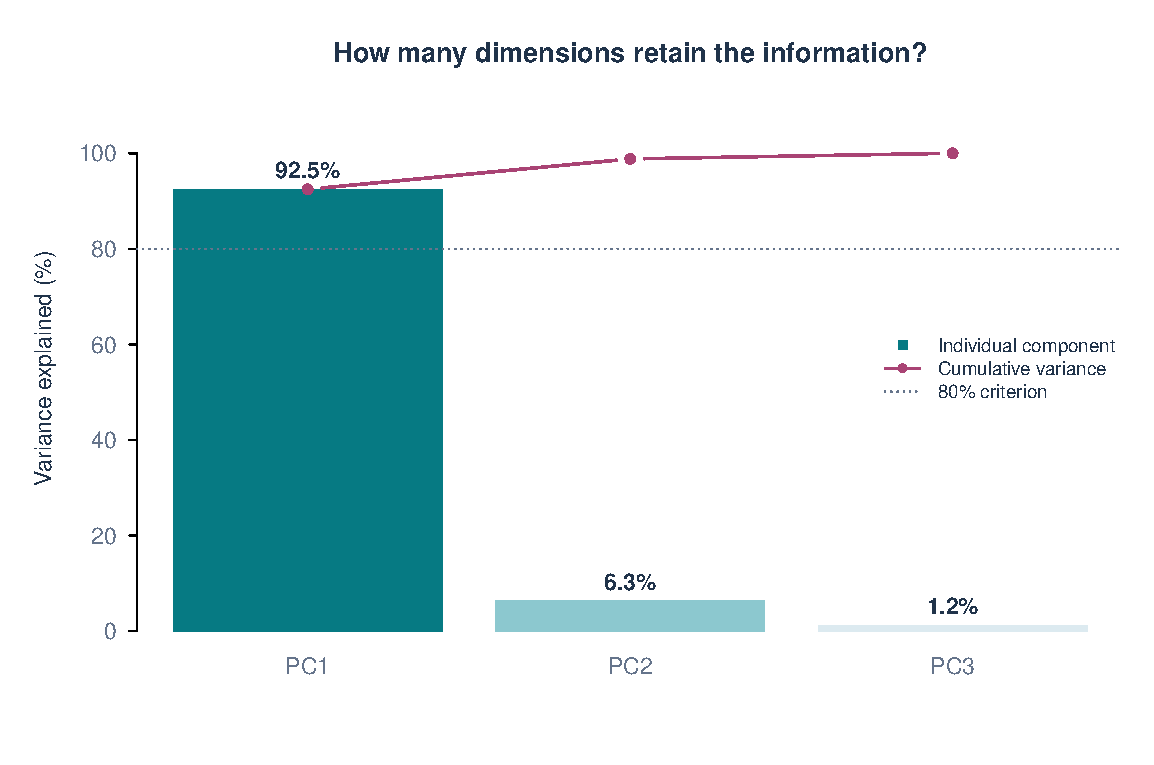
\includegraphics[width=\linewidth]{../figures/05_pca_scree.pdf}
\caption{Scree plot.}
\end{subfigure}\hfill
\begin{subfigure}[t]{0.53\textwidth}
\centering
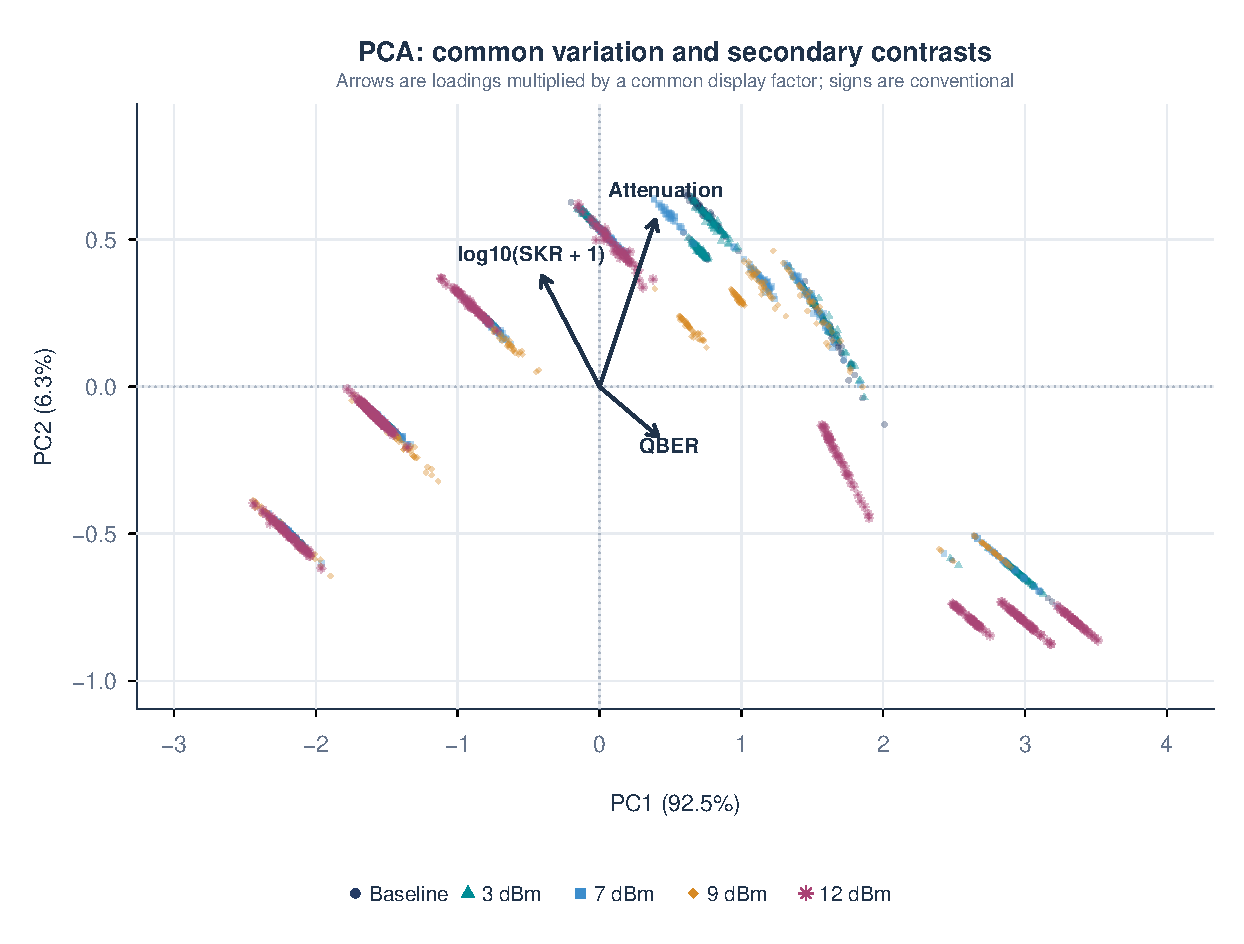
\includegraphics[width=\linewidth]{../figures/06_pca_biplot.pdf}
\caption{PC1--PC2 biplot.}
\end{subfigure}
\caption{PCA dimensionality and the geometry of the QKD observations. The biplot overlays variable loadings on observation scores.}
\label{fig:pca}
\end{figure}

The biplot should not be interpreted as a supervised classifier: the noise-condition labels are overlaid only after PCA is computed. Thus, any visible separation indicates that coexistence conditions correspond to naturally different regions of the measured multivariate performance space. Conversely, overlap indicates that attenuation-dependent QKD behavior can be similar across nearby injected-power conditions.

\section{Cluster Analysis}
\subsection{K-means Clustering}
K-means clustering was applied to the standardized quantitative variables. For a selected number of clusters $k$, the method minimizes the within-cluster objective
\[
\sum_{r=1}^{k}\sum_{\mathbf{z}_i\in C_r}\|\mathbf{z}_i-\boldsymbol{\mu}_r\|_2^2,
\]
where $\boldsymbol{\mu}_r$ is the centroid of cluster $C_r$. Models for $k=1,\ldots,10$ were fit with multiple random starts. The elbow curve was supplemented by a geometric knee estimate based on the point farthest from the chord joining the first and final WSS values. This selected $k=\KOptimal$ rather than forcing the number of clusters to equal the five known noise labels.

\begin{figure}[H]
\centering
\begin{subfigure}[t]{0.47\textwidth}
\centering
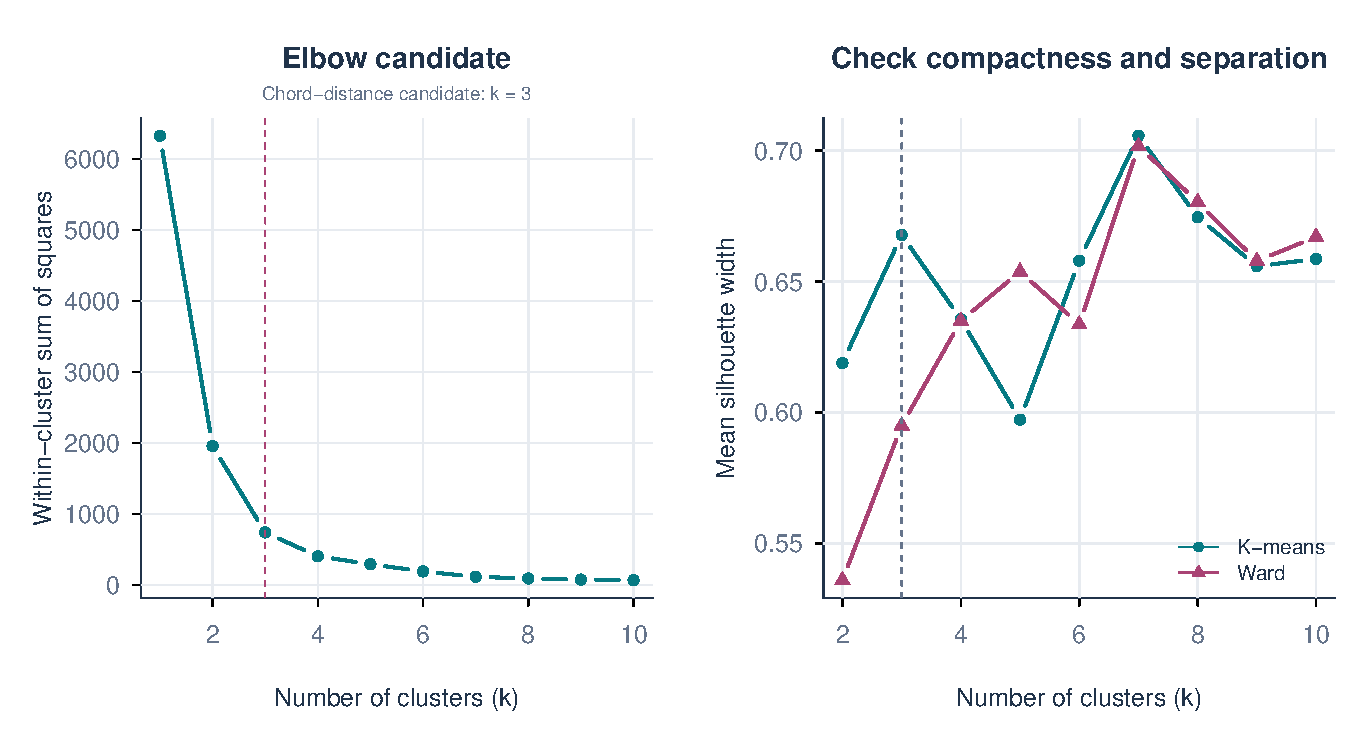
\includegraphics[width=\linewidth]{../figures/07_elbow_method.pdf}
\caption{Elbow analysis.}
\end{subfigure}\hfill
\begin{subfigure}[t]{0.51\textwidth}
\centering
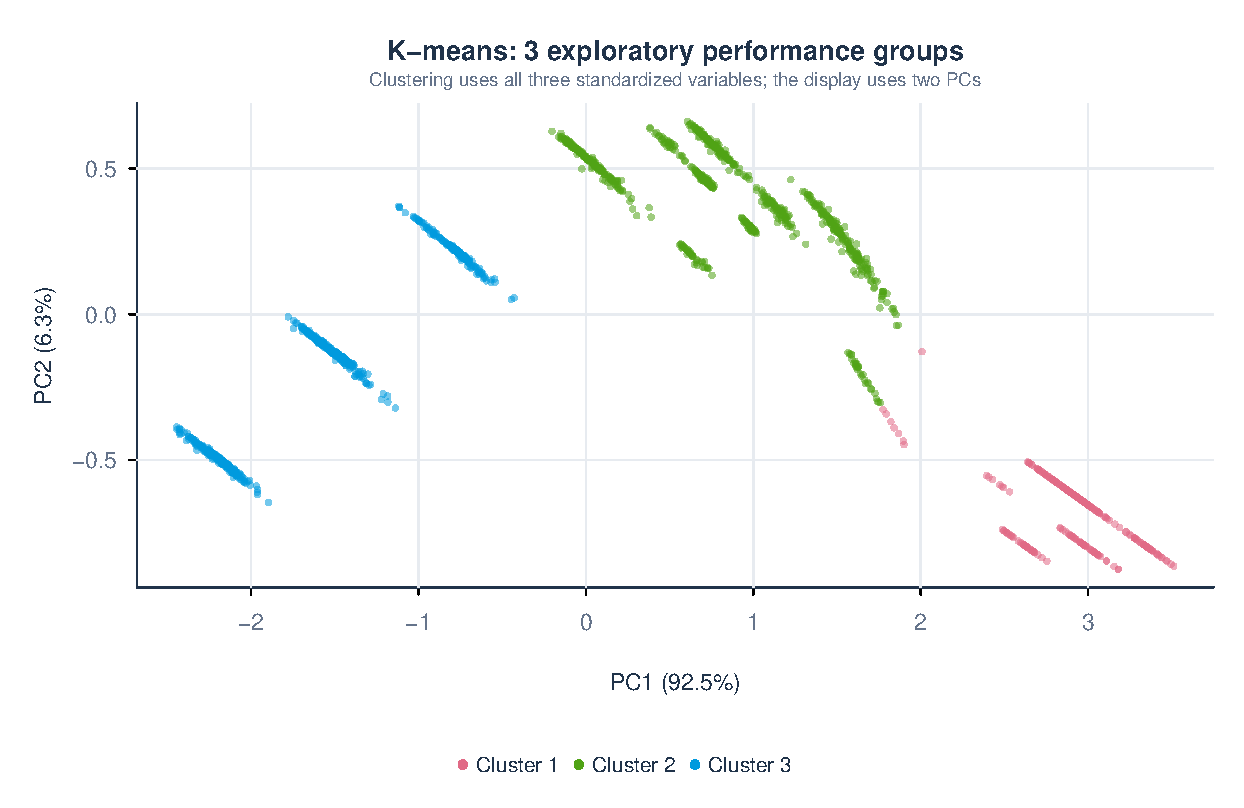
\includegraphics[width=\linewidth]{../figures/08_kmeans_clusters_pca.pdf}
\caption{K-means clusters in PCA space.}
\end{subfigure}
\caption{Selection and visualization of the K-means cluster solution.}
\label{fig:kmeans}
\end{figure}

The fact that the data-driven $k$ need not equal five is itself informative. K-means is unaware of the experimental condition labels and groups observations only by similarity in attenuation, QBER, and transformed SKR. Therefore, multiple injected-power conditions may occupy a common performance regime, while a single nominal condition can span more than one regime as attenuation increases toward link collapse.

\subsection{Hierarchical Clustering}
Agglomerative hierarchical clustering was performed with Euclidean distance on standardized variables and Ward's minimum-variance linkage. The dendrogram in Figure~\ref{fig:hier} shows the nested structure without requiring a fixed number of clusters in advance. For direct comparison with K-means, the tree was cut at $k=\KOptimal$.

\begin{figure}[H]
\centering
\begin{subfigure}[t]{0.56\textwidth}
\centering
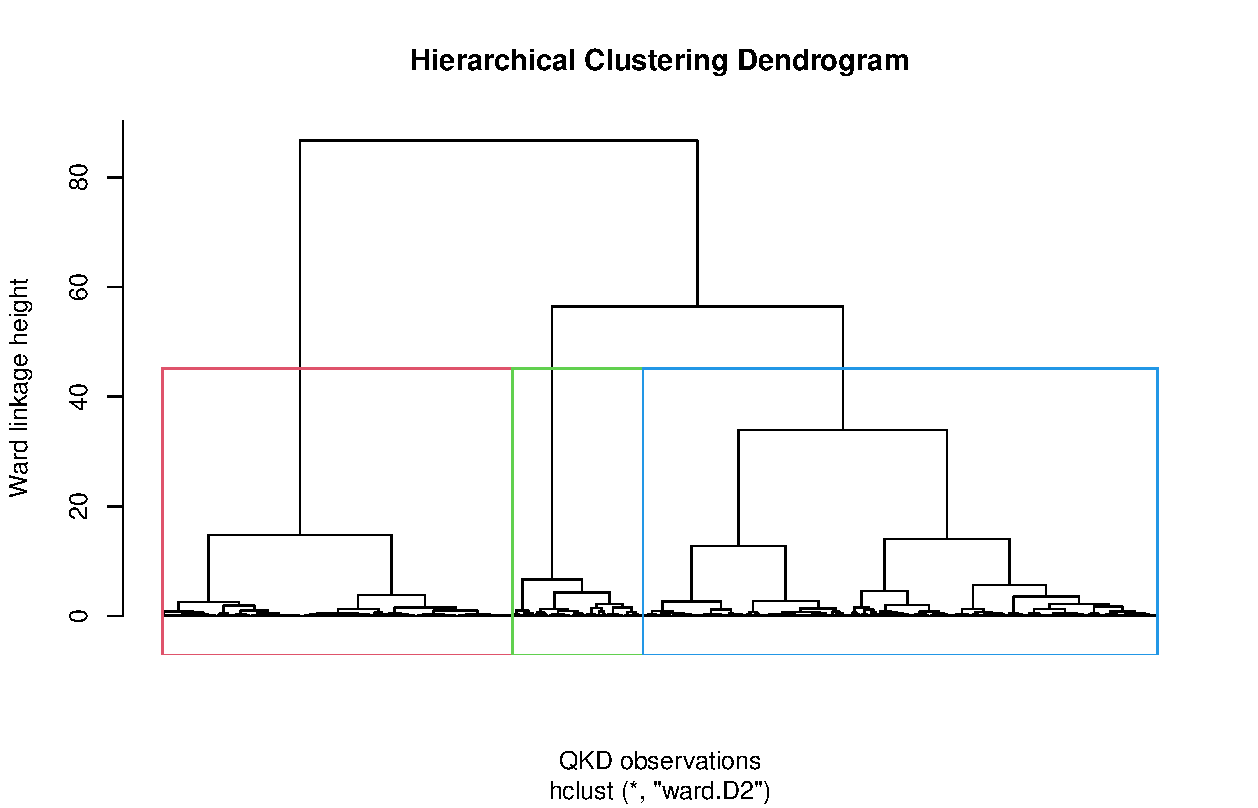
\includegraphics[width=\linewidth]{../figures/09_hierarchical_dendrogram.pdf}
\caption{Ward-linkage dendrogram.}
\end{subfigure}\hfill
\begin{subfigure}[t]{0.42\textwidth}
\centering
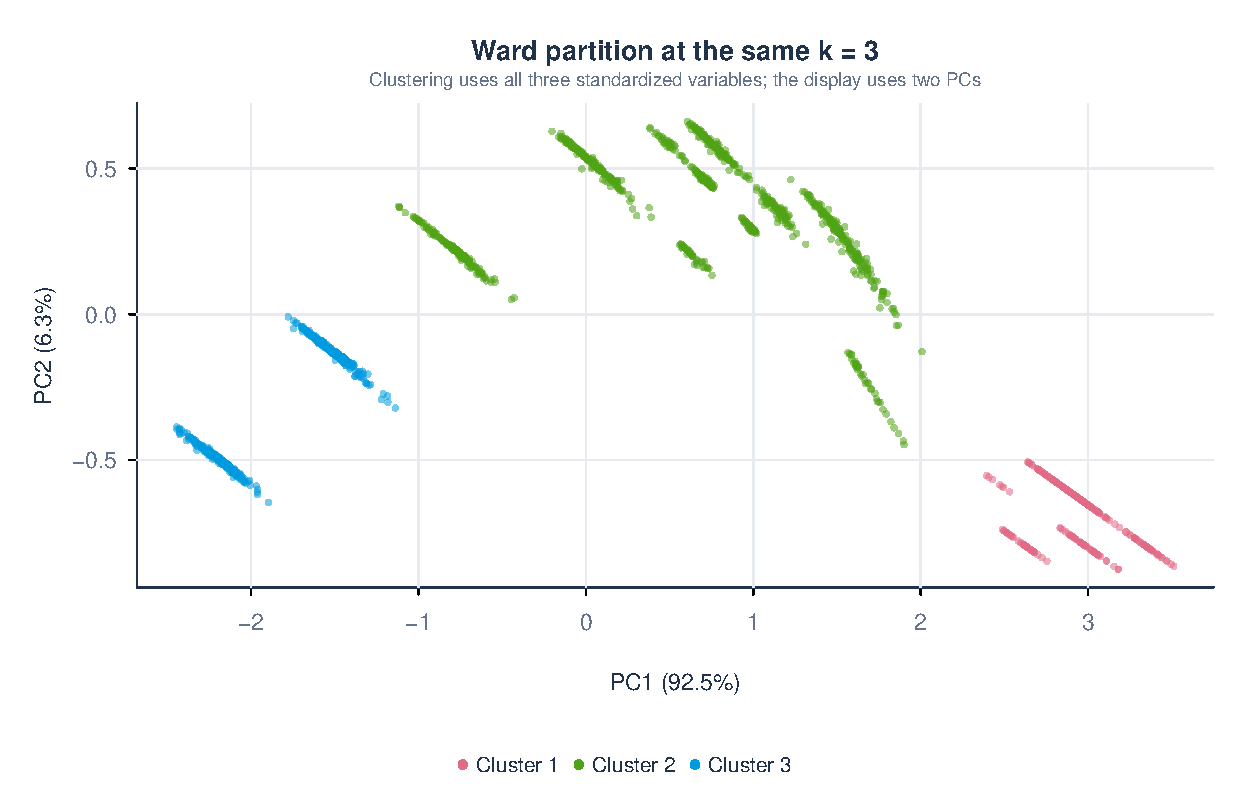
\includegraphics[width=\linewidth]{../figures/10_hierarchical_clusters_pca.pdf}
\caption{Tree cut visualized in PCA space.}
\end{subfigure}
\caption{Hierarchical clustering of the QKD measurements.}
\label{fig:hier}
\end{figure}

The PCA projections allow a visual comparison of the K-means and hierarchical partitions, but no formal agreement or stability measure is reported. Apparent similarities are therefore exploratory evidence of possible performance regimes. Differences between the two methods are also expected: K-means favors approximately centroid-shaped groups, whereas Ward linkage constructs clusters from a sequence of local merges. Cluster membership describes similarity in the measured variables and does not establish independent physical states or replace the known experimental labels.

\section{Linear Discriminant Analysis}
LDA was used as the supervised counterpart to PCA and clustering. The predefined response variable was injected-signal condition with five classes. Predictors were standardized attenuation, QBER, and transformed SKR. To evaluate classification beyond resubstitution accuracy, each class was split approximately 70/30 into training and held-out test observations using a fixed random seed. The resulting model used \TrainN{} training observations and \TestN{} held-out observations.

LDA seeks linear combinations
\[
LD_j = a_{j1}z_{\mathrm{VOA}} + a_{j2}z_{\mathrm{QBER}} + a_{j3}z_{\log(\mathrm{SKR}+1)}
\]
that maximize separation among predefined groups relative to within-group variation. Standardizing with training-set means and standard deviations puts the coefficients on a common predictor scale. Their magnitudes describe conditional contributions within each discriminant direction; correlated predictors mean that these magnitudes are not independent measures of variable importance. The largest absolute coefficient on LD1 corresponds to \texttt{\LDOneTop}; on LD2 it is \texttt{\LDTwoTop}.

\begin{table}[H]
\centering
\caption{LDA scaling coefficients for standardized predictors.}
\label{tab:lda_coef}
\small
\IfFileExists{../results/lda_coefficients_table.tex}{\begin{tabular}{lrrr}
\toprule
Predictor & LD1 & LD2 & LD3 \\
\midrule
VOA\_dB & 0.907 & 1.929 & 0.005 \\
QBER & 2.456 & -3.406 & -0.488 \\
LogSKR & 3.236 & -1.730 & 0.528 \\
\bottomrule
\end{tabular}
}{Results generated when the R analysis runs.}
\end{table}

\begin{figure}[H]
\centering
\begin{subfigure}[t]{0.51\textwidth}
\centering
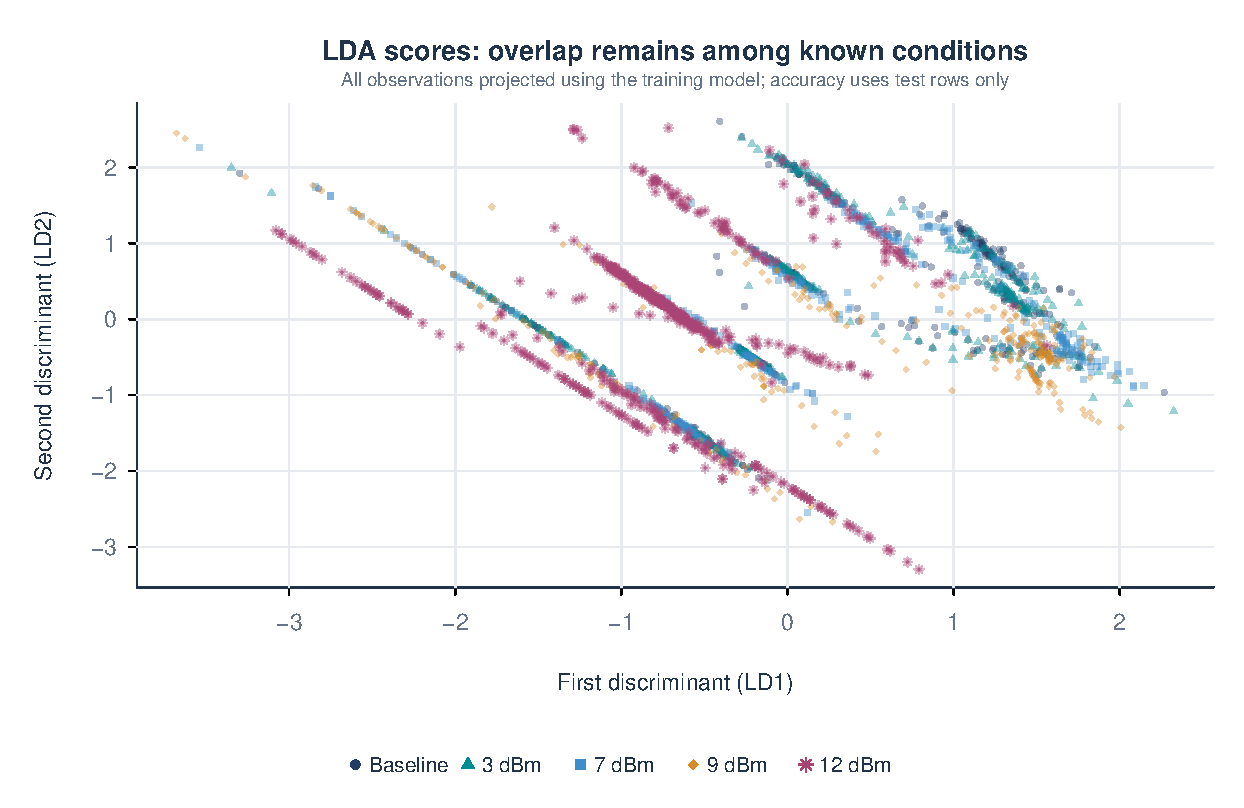
\includegraphics[width=\linewidth]{../figures/11_lda_separation.pdf}
\caption{First two discriminant dimensions.}
\end{subfigure}\hfill
\begin{subfigure}[t]{0.47\textwidth}
\centering
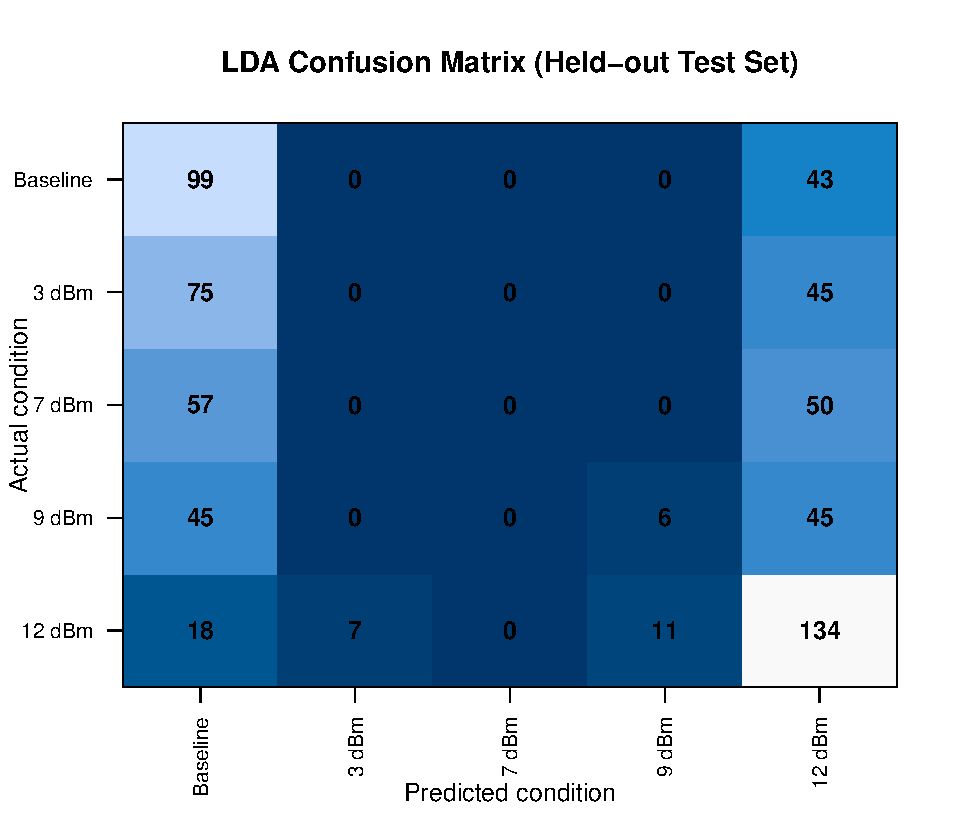
\includegraphics[width=\linewidth]{../figures/12_lda_confusion_matrix.pdf}
\caption{Held-out confusion matrix.}
\end{subfigure}
\caption{Supervised separation and classification performance of LDA.}
\label{fig:lda}
\end{figure}

\begin{table}[H]
\centering
\caption{Held-out LDA classification counts.}
\label{tab:conf}
\small
\IfFileExists{../results/lda_confusion_table.tex}{\begin{tabular}{lrrrrr}
\toprule
Actual $\backslash$ Pred. & Baseline & 3 dBm & 7 dBm & 9 dBm & 12 dBm \\
\midrule
Baseline & 99 & 0 & 0 & 0 & 43 \\
3 dBm & 75 & 0 & 0 & 0 & 45 \\
7 dBm & 57 & 0 & 0 & 0 & 50 \\
9 dBm & 45 & 0 & 0 & 6 & 45 \\
12 dBm & 18 & 7 & 0 & 11 & 134 \\
\bottomrule
\end{tabular}
}{Results generated when the R analysis runs.}
\end{table}

The held-out classification accuracy is \textbf{\LDAAccuracy}. Misclassifications should be read alongside the LD1--LD2 plot: overlap between adjacent coexistence conditions indicates that the measured performance variables do not uniquely encode injected power at every attenuation. This is physically plausible because attenuation itself changes QBER and SKR, creating partially overlapping performance states. LDA nevertheless quantifies how much of the predefined coexistence condition can be recovered from the joint measurement vector.

This accuracy measures prediction of held-out rows within the same experimental campaign. Measurements at shared attenuation and noise settings can occur in both partitions, and repeated measurements may be dependent. The estimate does not establish performance on independent experimental runs or previously unseen operating settings; validation grouped by run or experimental setting would be needed to assess that broader generalization. LDA also assumes common within-class covariance and approximately Gaussian class-conditional predictors, assumptions that bounded QBER and zero-heavy SKR may not satisfy.

\section{Conclusion}
This analysis demonstrates how complementary multivariate methods reveal different aspects of experimental QKD coexistence data. PCA summarizes the dominant joint variation of attenuation, QBER, and secure key rate, while K-means and hierarchical clustering identify unlabeled performance regimes without assuming that they must match the five experimental conditions. LDA then uses the known injected-signal labels to quantify supervised group separation and achieves \LDAAccuracy{} accuracy on held-out observations. Taken together, the results show that QKD performance under classical-signal coexistence is inherently multivariate: attenuation, error behavior, and usable key throughput should be interpreted jointly rather than as isolated metrics.

\section*{Reproducibility Note}
All preprocessing, statistical analyses, tables, and figures in this report are generated by the accompanying R script. The script downloads the cited Zenodo CSV files, retains the \SI{0}{km} coexistence measurements, preserves physically meaningful zero-SKR observations, and uses a fixed random seed (2026) for K-means initialization and the LDA train/test split.

\begin{thebibliography}{9}
\bibitem{horgan2026}
J. Horgan, N. Quigley, B. Hajar, D. Briantcev, A. Kaszubowska-Anandarajah, and D. Kilper,
``QKD Network Characterisation and Coexistence Datasets with Standardised Performance Metrics and Experimental Methods,''
Zenodo, version 2, 2026. DOI: \href{https://doi.org/10.5281/zenodo.21792844}{10.5281/zenodo.21792844}.

\bibitem{rproject}
R Core Team, \emph{R: A Language and Environment for Statistical Computing}. R Foundation for Statistical Computing, Vienna, Austria.

\bibitem{mass}
W. N. Venables and B. D. Ripley, \emph{Modern Applied Statistics with S}, 4th ed. Springer, 2002.
\end{thebibliography}

\end{document}
